%************************************************
\section{White-box Model}\label{ch:Whitebox}
%************************************************

While a black-box analysis is very useful for systems where we do not have access to the source code, when we do have that access
it would be a waste not to work with this additional information. Now instead of a black-box analysis we can use a white-box analysis 
that takes advantage of these new information and uses them to derive a result differently then the black-box approach.


\begin{figure}[h]
    \centering
    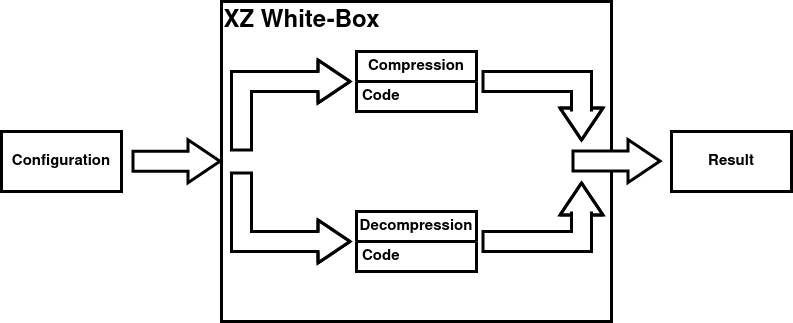
\includegraphics[scale=0.6]{gfx/XZWhitebox.png}
    \caption{A White-box Version of XZ}
    \label{fig:WBxz}
\end{figure}

Let us now inspect our example \autoref{fig:xz} from a white-box perspective


We are aware of the inner workings of the system, and given the system an input we can observe how the system uses the input, which functions are called, 
in what capacity a feature influence the program flow. 

We use these newly available information to formulate a model that differs from our black-box approach, instead of only measuring the time the system
needs to finish the process and use the input data to infer in what capacity each feature influences the system. 

\subsection{Disadvantages of White-Box}
When using white-box model we clearly see how a feature interacts with another feature, due to that we do not need to sample our configuration space like
we do in the black-box, meaning we do not face the problem of combinatorial explosion. 
Neither do we have to handle multicollinearity features differently, since we can see in what extend they influence each other. 
The example from \ref{ColinearF} would be no problem for the white-box model since we are aware that $c$ and $d$ do not interact with one another and can
therefore assign them the precise amount of time they spend in their code region respectively, whereas the black-box model needs to infer this information.

With the surplus of information, the white-box model faces different challenges. 
First and foremost, to analyze larger systems we need a robust strategy and in depth code comprehension.

\subsubsection{Analyzing Strategies}
Analyzing programs is a highly complex topic in itself, it is not a trivial task to use a program to run a analysis over a different system.
In our case, we first need to find out which parts of the code corresponds to which feature.

To solve this problem multiple solutions have been proposed, Weber et. al. \cite{White-box-Profiling} uses a profiling approach, to generate 
performance-influence models that depict configurability on a method level, to achieve this they first used a JProflier a coarse-grained profiler
to learn a performance influence model for every method that have been learned successfully. 
To identify the methods that are hard to learn they use a filtering techniques, afterwards using KIEKER a fine-grained profiler to learn these methods.

Velez et. al. introduced us to ConfigCrusher \cite{ConfigCrusher} a white-box analysis, that uses a static data-flow analysis to see how features influence 
variables and the control-flow of the system. In addition, ConfigCrusher uses three insights about configurable systems, from previous works, namely
irrelevance, orthogonality and low interaction degree. Irrelevance, is used to identify the features that are relevant for the data-flow of the system, and by
doing so reducing the amount of configurations necessary to analyze the system. Orthogonality, is used to identify features that do not influence each other, and
thus can be measured together. Low interaction degree, is used to identify the relevant feature interaction, since only few features interact with another, 
ConfigCrusher focuses on those configurations with interacting features to reduce the amount of configuration that need to be sampled.

Siegmund et. al. introduced us to Comprex \cite{Comprex} which uses a dynamic taint analysis to identify how
and to what degree features influence the control-flow of the given system. 
To reduce measurement costs they introduce two techniques, namely compression and composition. 
Compression is used to reduce the number of configurations necessary to analyze the system,
by simultaneously analyzing regions that are independent of another, therefore they can use a single configuration to 
analyze different features. 
They take advantage of the fact that \perfInfluenceModel can be build compositionally, by generating a performance-influcence model for each region separately
and afterwards compose all the local \perfInfluenceModel into a model for the whole system.

Both Comprex and ConfigCrusher use the techniques of compression and composition, the major difference between both analysis methods is Comprex uses a dyanmic taint
analysis, whereas ConfigCrusher uses a static data-flow analysis. 


After figuring out which parts of the code corresponds to what feature we still need to instrumentalize the code 

\subsection{Indepth Code comprehension} %Title work in progress